
	\begin{enumerate}
		\item Дата собрания : 16.09.14
		\item Цель:
		\begin{itemize}
			\item Собрать основу робота, а именно колесную базу
			\item Написать простейшую программу для управления роботом
		\end{itemize}			
		\item Реализация :
		\begin{itemize}
			\item Была собрана квадратная конструкция(Рис. 1)
			\item Написана программа для передвижения
		\end{itemize}
		\item Результаты
		\begin{itemize}
			\item Собран четырехколесный робот, способный передвигаться по четырем направлениям
			\item Робот управляется с помощью геймпада
		\end{itemize}
		Получившаяся конструкция:
		\begin{figure} [h]
			\centering
			\begin{minipage}{0.3\linewidth}
				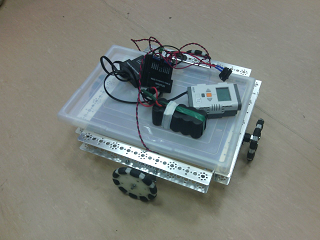
\includegraphics[width=35mm,height=35mm]{/!my_data/projects/pml30-psi_team/Days/16.09.14/1_1_robot.png}\\ Рисунок 1
			\end{minipage}
			\begin{minipage}{0.3\linewidth}
				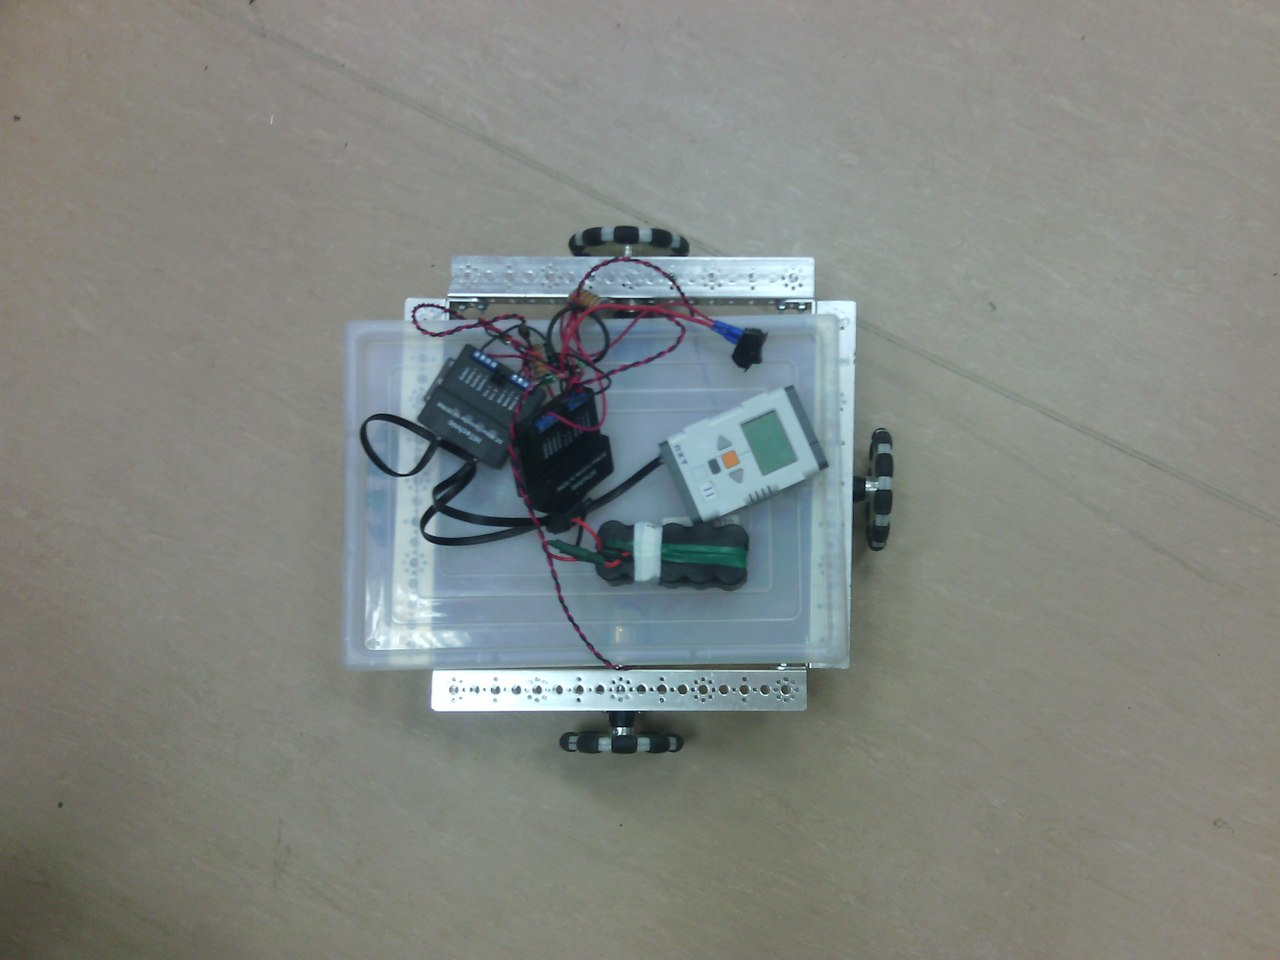
\includegraphics[width=35mm,height=35mm]{/!my_data/projects/pml30-psi_team/Days/16.09.14/1_2_robot}\\ Рисунок 2
			\end{minipage}
		\end{figure}
	\end{enumerate}